\documentclass[12pt]{article}
\usepackage{preamble}
\usepackage{longtable}

\geometry{a4paper, left=2.5cm, right=2.5cm, top=2cm, bottom=2.5cm}

\pagestyle{plain}

\newcommand{\placeholder}[1]{{\color{magenta}#1}}

\chead{
    \begin{minipage}{1\linewidth}
        \begin{wrapfigure}{r}{0pt}
            
\includegraphics[height=1cm]{images/logo}
        \end{wrapfigure}
        {
            \centering
            \sffamily\scriptsize
            \textbf{
                Санкт-Петербургский национальный исследовательский университет \\
                информационных технологий, механики и оптики}
            %th3p4g
            \vspace{2mm}

            \quad\quad\quad\quad\quad\quad\ \textbf{УЧЕБНЫЙ ЦЕНТР ОБЩЕЙ ФИЗИКИ ФТФ}
        }
    \end{minipage}
}



\begin{document}
    \vspace*{2\baselineskip}

    \thispagestyle{fancy}

    \noindent
    \textbf{Группа} \underline{M3200\hspace{4.5cm}} \hfill \textbf{К работе допущен} \underline{\hspace{4cm}} \\[0.5cm]
    \textbf{Студенты} \underline{Комашко А., Семёнов Д.\hspace{0.45cm}} \hfill \textbf{Работа выполнена} \underline{\hspace{4cm}} \\[0.5cm]
    \textbf{Преподаватель} \underline{Шоев В. И.\hspace{1.9cm}} \hfill \textbf{Отчет принят} \underline{\hspace{4.85cm}} \\



    \begin{center}
    {\huge \textbf{Рабочий протокол и отчёт по\\ лабораторной работе № 3.07}}

        \smallvspace

        {\Large Изучение свойств ферромагнетика}
    \end{center}


    \noindent
    1. \textbf{Цель работы.}

    \begin{enumerate}
        \item Измерение зависимости магнитной индукции в ферромагнетике от напряженности магнитного поля $B = B(H)$
        \item Определение по предельной петле гистерезиса индукции насыщения, остаточной индукции и коэрцитивной силы
        \item Получение зависимости магнитной проницаемости от напряженности магнитного поля $\mu = \mu(H)$ и оценка максимального значения величины магнитной проницаемости
        \item Расчет мощности потерь энергии в ферромагнетике в процессе его перемагничивания
    \end{enumerate}

    \mediumvspace

    \noindent
    2. \textbf{Задачи, решаемые при выполнении работы.}

    \begin{enumerate} 
        \item Измерение значений параметров предельной петли гистерезиса.
        \item Построение кривой начального намагничивания $B_m = B_m(H_m)$ и графика зависимости магнитной проницаемости $\mu = \mu(H)$ от напряженности магнитного поля
        \item Вычисление максимального значения магнитной проницаемости
    \end{enumerate}

    \mediumvspace

    \noindent
    3. \textbf{Объект исследования: } 

    Для изучения магнитных свойств ферромагнитного материала выбран сердечник (магнитопровод) трансформатора. Объект измерений имеет прямоугольную форму с прямоугольным же поперечным сечением.

    \mediumvspace

    \noindent
    4. \textbf{Метод экспериментального исследования.}

    Прямые и косвенные измерения параметров предельной петли гистерезиса при изменении амплитудных значений напряжённости и индукции магнитного поля.

    \mediumvspace

    \noindent
    5. \textbf{Рабочие формулы и исходные данные.}

    \text{Индукция магнитного поля в некотором материале}
\[
    \vec{B} = \mu_0(\vec{H} + \vec{J})
\]

\text{Где:}
\begin{center}
    $\vec{H} - \text{напряжённость магнитного поля}$ \\
    $\vec{J} - \text{намагниченность материала}$ \\
    $\mu_0 = 4\pi \cdot 10^{-7} \frac{\text{Гн}}{\text{м}} - \text{магнитная постоянная}$
\end{center}

\text{Зависимость магнитной проницаемости материала}
\[
    \mu = 1 + \frac{J}{H} = \frac{B}{\mu_0 H}
\]

\text{Теорема о циркуляции напряженности магнитного поля}
\[
    \oint H d\ell = N_1 \cdot I_1
\]

\text{Где:}
\begin{center}
    $N_1 - \text{число витков на намагничивающей (первичной) обмотке образца}$ \\
    $I_1 - \text{сила тока образца}$
\end{center}

\text{Напряженность магнитного поля}
\[
    H = \frac{N_1}{\ell} \cdot I_1 = \frac{N_1}{\ell R_1} \cdot K_x \cdot x = \alpha \cdot K_x \cdot x
\]

\text{Где:}
\begin{center}
    $x - \text{координата по горизонтальной оси OX экрана осциллографа}$ \\
    $K_x - \text{цена деления горизонтальной шкалы}$
\end{center}

\text{Электродвижущая сила во вторичной обмотке по Закону Фарадея}
\[
    \mathscr{E} = N_2 \left| \frac{\partial \Phi}{\partial t} \right| = N_2 S \left| \frac{dB}{dt} \right|
\]

\text{Где:}
\begin{center}
    $N_2 - \text{число витков на вторичной обмотке образца}$
\end{center}

\text{Индукция магнитного поля в образце}
\[
    B = \frac{1}{N_2 S} \int{\mathscr{E}}dt
\]

\text{Напряжение на интегрирующей RC-цепочке}
\[
    U_C = \frac{1}{R_2 C_1} \int{\mathscr{E}}dt
\]

\text{Связь напряжения конденсатора с магнитной индукцией}
\[
    U_C = \frac{N_2 S}{R_2 C_1} \cdot B
\]

\text{Связь индукции и вертикального размера осцилограммы}
\[
    B = \frac{R_2 C_1}{N_2 S}\cdot K_y \cdot y = \beta \cdot K_y \cdot y  
\]

\text{Где:}
\begin{center}
    $x - \text{координата по вертикальной оси OX экрана осциллографа}$ \\
    $K_x - \text{цена деления вертикальной шкалы}$
\end{center}

\text{Формула для расчета потерь энергии в ферромагнетике}
\[
    P = \chi \cdot S_{\text{ПГ}}
\]

\text{Где:}
\begin{center}
    $S_\text{ПГ} - \text{площадь петли гистерезиса}$
\end{center}

\text{Коэффициент $\chi$}
\[
    \chi = K_x K_y\frac{N_1 R_2 C_1}{N_2 R_1}f
\]

\text{Где:}
\begin{center}
    $f - \text{частота сигнала, подаваемого на первичную обмотку трансформатора}$
\end{center}

\text{Элементарная работа по перемагничиванию единицы объёма}
\[
    dA = V \cdot H dB
\]

\text{Полная работа по перемагничиванию единицы объема}
\[
    \frac{A}{V} = \frac{1}{V} \oint dA = \oint H dB
\]

\textbf{Исходные данные}
\begin{center}
    $N_1 = 1665$ - число витков на первичной обмотке образца. \\
    $N_2 = 970$ - число витков на вторичной обмотке образца. \\
    $\ell = 7,8 \pm 0,1$ см - средняя длина ферромагнетика. \\
    $S = 0,64 \pm 0,05$ см$^2$ - площадь поперечного сечения ферромагнетика. \\
    $R_1 = 68 \pm 10\%$ Ом \\
    $R_2 = 470 \pm 10\%$ кОм \\
    $C_1 = 0,47 \pm 10\%$ мкФ \\
    $f = 35$ Гц - частота сигнала, \\ подаваемого на первичную обмотку трансформатора
\end{center}

    \mediumvspace

    \newpage

    \noindent
    6. \textbf{Измерительные приборы.}

    \smallvspace

    \begin{center}
    \begin{tabular}{|c|m{5cm}|C{2cm}|C{2cm}|C{2cm}|c|}
        \hline
        № п/п & Наименование            & Тип\newlineприбора & Предел\newlineизмерений & $\Delta_n$ \\
        \hline
        1 & Цифровой запоминающий осциллограф GDS-71102B & Цифровой & 0 - 20 В & 0,1 В    \\
        \hline
        2 & Генератор сигналов АКИП-3409/2 & Цифровой & 20 - 40 Гц & 0,1 Гц \\
        \hline

    \end{tabular}

    \smallvspace

    \textit{Таблица 1.} Измерительные приборы
\end{center}

    \mediumvspace

    \noindent
    7. \textbf{Схема установки. (перечень схем, которые составляют Приложение 1).}

    \hyperlink{schema1}{Схема установки} прилагается в Приложении 1

    \mediumvspace

    \noindent
    8. \textbf{Результаты прямых измерений и их обработки (таблицы, примеры расчетов).}

    \begin{itemize}
    \item Прилагаются \hyperlink{table2}{Таблица 2}, \hyperlink{table2}{Таблица 3}, \hyperlink{table2}{Таблица 4}  в Приложении 2

    \smallvspace

    \item Расчёт масштабирующих коэффициентов $\alpha$ и $\beta$: \\
    $\alpha = \frac{N_1}{\ell R_1} = \frac{1665}{0,078 \cdot 68} = 313,914 (\text{м} \cdot \text{Ом})^{-1}$ \\
    $\beta = \frac{R_2 C_1}{N_2 S} = \frac{47000 \cdot 4,7 \cdot 10^{-7}}{970 \cdot 6,4 \cdot 10^{-5}} = 3,558 \frac{\text{Ом} \cdot \text{Ф}}{\text{м}^2}$
    
    \smallvspace

    \item Расчёт коэрцитивной силы $H_c$ и остаточной индукции $B_r$: \\
    $H_c = \alpha \cdot K_x \cdot X_c = 313,914 \cdot 0,1 \cdot 1 = 31,391 \frac{\text{А}}{\text{м}}$ \\
    $B_r = \beta \cdot K_y \cdot Y_r = 3,558 \cdot 0,05 \cdot 1,4 = 0,249 \text{Тл}$

    \smallvspace

    \item Расчёт напряжённости $H_m$ и индукции $B_m$ магнитного поля, магнитной проницаемости $\mu$: \\
    $H_m = \alpha \cdot K_x \cdot X_m = 313,914 \cdot 0,1 \cdot 2,7 = 84,757 \frac{\text{А}}{\text{м}}$ \\
    $B_m = \beta \cdot K_y \cdot Y_m = 3,558 \cdot 0,05 \cdot 2,3 = 0,409 \text{Тл}$ \\
    $\mu = \frac{B_m}{\mu_0 H_m} = \frac{0,409}{4 \cdot \pi \cdot 10^{-7} \cdot 84,757} = 3842$

    \smallvspace

    \item Расчёт коэффициента $\chi$: \\
    $\chi = K_x K_y\frac{N_1 R_2 C_1}{N_2 R_1}f = 0,1 \cdot 0,05 \cdot \frac{1665 \cdot 470000 \cdot 4,7 \cdot 10^{-7}}{970 \cdot 68} \cdot 35 = 9,8 \cdot 10^{-4} \frac{\text{Дж}}{\text{с}}$

    \smallvspace

    \item Расчёт площади петли гистерезиса ферромагнетика $S_{\text{ПГ}}$: \\
    Сделаем интерполяцию верхней и нижней кривой петли гистерезиса при помощи полиномов Лагранжа $8$ степени: \\
    $y_{\text{верхн.}}(x) = -\frac{112694375}{70563397632}x^{8}+\frac{1581874625}{211690192896}x^{7}+\frac{64101575}{2520121344}x^{6}-\frac{234701845}{1890091008}x^{5}-\frac{3018111}{52502528}x^{4}+\frac{160856177}{295326720}x^{3}-\frac{126896811}{287123200}x^{2}+\frac{242428759}{538356000}x+\frac{3}{2}$ \\
    $y_{\text{нижн.}}(x) = \frac{889124375}{211690192896}x^{8}+\frac{264950125}{23521132544}x^{7}-\frac{141572225}{2520121344}x^{6}-\frac{31610635}{210010112}x^{5}+\frac{9677683}{52502528}x^{4}+\frac{4758729}{8203520}x^{3}+\frac{279651061}{1292054400}x^{2}+\frac{9812577}{22431500}x-\frac{7}{5}$ \\

    $S_{\text{ПГ}} = \int_{-3,2}^{2,7}(y_{\text{верхн.}}(x) - y_{\text{нижн.}}(x))dx = 8,425 \text{дел.}^2$

    \smallvspace

    \item Расчёт средней мощности $P$, расходуемой на перемагничивание образца: \\
    $P = \chi \cdot S_{\text{ПГ}} = 9,8 \cdot 10^{-4} \cdot 8,425 = 8,22 \cdot 10^{-3} \text{Вт}$

    \smallvspace

    \item Максимум магнитной проницаемости материала $\mu_{max} = 4655,66$ достигается при напряжённости поля $H = 48,657 \frac{\text{А}}{\text{м}}$
    
    
\end{itemize}


    \mediumvspace

    \noindent
    
    9. \textbf{Расчёт погрешности измерений.}
    
    \begin{itemize}
    \item Расчёт погрешности найденной величины мощности потерь на перемагничивание ферромагнетика: \\
    $\varepsilon_{\chi} = \frac{\Delta \chi}{\chi}\cdot 100\%\;\approx\;\sqrt{
        \Bigl(\frac{\Delta K_x}{K_x}\Bigr)^2
        \;+\;
        \Bigl(\frac{\Delta K_y}{K_y}\Bigr)^2
        \;+\;
        \Bigl(\frac{\Delta R_2}{R_2}\Bigr)^2
        \;+\;
        \Bigl(\frac{\Delta C_1}{C_1}\Bigr)^2
        \;+\;
        \Bigl(\frac{\Delta R_1}{R_1}\Bigr)^2
        \;+\;
        \Bigl(\frac{\Delta f}{f}\Bigr)^2}\cdot 100\%$ \\
    
    $\varepsilon_{\chi}\;\approx\;\sqrt{
        1^2 + 1^2 + 10^2 + 10^2 + 10^2 + 1^2
        }\;\approx\;17,32\%$ \\

    $\varepsilon_{P} = \frac{\Delta P}{P}\cdot100\%\;\approx\;\sqrt{
        \Bigl(\frac{\Delta \chi}{\chi}\Bigr)^2
        \;+\;
        \Bigl(\frac{\Delta S_{\text{ПГ}}}{S_{\text{ПГ}}}\Bigr)^2}\cdot100\%\;\approx\;\sqrt{
        17,32^2 \;+\;10^2
        }\;\approx\;20\%$ \\
    
\end{itemize}

    \mediumvspace

    \noindent
    10. \textbf{Графики (перечень графиков, которые составляют Приложение 3).}

    \begin{itemize}
        \item \hyperlink{diagram1}{Кривая начального намагничивания $B_m = B_m(H_m)$}
        \item \hyperlink{diagram2}{Зависимость магнитной проницаемости $\mu = \mu(H_m)$ от напряженности магнитного поля}
        \item \hyperlink{diagram3}{Петля гистерезиса ферромагнетика}
        \item \hyperlink{diagram4}{Интерполяция петли гистерезиса ферромагнетика}
    \end{itemize}

    \mediumvspace

    \noindent
    11. \textbf{Окончательные результаты.}

    \begin{itemize}
    \item Значение коэрцитивной силы, остаточной индукции и магнитной проницаемости в состоянии насыщения: \\
    $B_r = 0,249 \text{Тл}$ \\
    $H_c = 31,391 \frac{\text{А}}{\text{м}}$ \\
    $\mu = 3842$

    \item Мощность потерь на перемагничивание ферромагнетика (с оценкой величины ее погрешности): \\
    $P = (8,22 \pm 1,64) \cdot 10^{-3} \text{Вт}$

    \item Графики зависимостей магнитной индукции и проницаемости от напряженности в \textbf{Приложении 3}

    \item  Максимум магнитной проницаемости материала $\mu_{max} = 4655,66$ достигается при напряжённости поля $H = 48,657 \frac{\text{А}}{\text{м}}$
\end{itemize}

    \mediumvspace

    \noindent

    \newpage
    
    12. \textbf{Выводы и анализ результатов работы.}

    В ходе данной лабораторной работы была измерена зависимость магнитной индукции от напряжённости поля для исследуемого ферромагнетика. Измерения по предельной петле гистерезиса позволили определить следующие характеристики: коэрцитивная сила, остаточная индукция и магнитная проницаемость. Были построены графики зависимостей магнитной индукции и проницаемости от напряженности, они соответствуют теоретическому ожиданию.

    \clearpage

    \begin{center}
        \LARGE
        \textbf{Приложение 1. Схема установки}
    \end{center}

    \mediumvspace

    \hypertarget{schema}{}

\begin{center}
    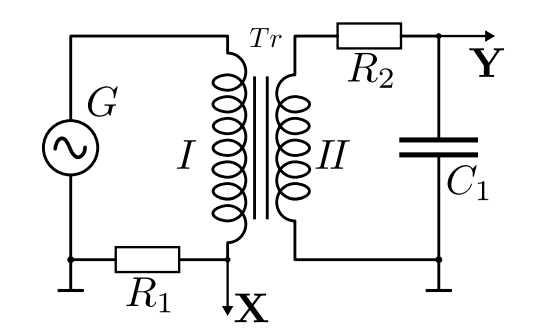
\includegraphics[width=15cm]{images/scheme1}

    \smallvspace

    \textit{Рисунок 1.} Принципиальная электрическая схема установки
\end{center}






    \clearpage

    \begin{center}
        \LARGE
        \textbf{Приложение 2. Таблицы измерений и расчётов}
    \end{center}

    \mediumvspace

    \begin{center}
    \hypertarget{table2}{}

    \renewcommand{\arraystretch}{1.8}

    \begin{tabular}{|C{2.5cm}|C{2.5cm}|C{2.5cm}|C{2.5cm}|}
        \hline
        $X_c$, дел & $Y_r$, дел & $H_c$, А/м & $B_r$, Тл  \\
        \hline
        1 & 1,4 & 31,391 & 0,249 \\
        \hline
    \end{tabular}

    \smallvspace

    \textit{Таблица 2.}

\end{center}

    \begin{center}
    \hypertarget{table3}{}

    \renewcommand{\arraystretch}{1.8}

    \begin{tabular}{|C{2.5cm}|C{2.5cm}|C{2.5cm}|C{2.5cm}|C{2.5cm}|}
        \hline
        $X_m$, дел & $Y_m$, дел & $H_m$, А/м & $B_m$, Тл & $\mu_m$  \\
        \hline
        2,7 & 2,3 & 84,757 & 0,409 & 3842 \\
        \hline
    \end{tabular}

    \smallvspace

    \textit{Таблица 3.}

\end{center}

    \begin{center}
    \hypertarget{table4}{}

    \renewcommand{\arraystretch}{1.8}

    \begin{tabular}{|C{1.7cm}|C{1.7cm}|C{1.7cm}|C{1.7cm}|C{1.7cm}|C{1.7cm}|C{1.7cm}|C{1.7cm}|}
        \hline
        $U$, В & $X$, дел & $K_x$, В/дел & $H$, А/м & $Y$, дел & $K_y$, В/дел & $B$, Тл & $\mu$  \\
        \hline
        20,00 & 2,7 & 0,1 & 84,757 & 2,3 & 0,05 & 0,409 & 3842,00 \\
        \hline
        19,25 & 2,6 & 0,1 & 81,618 & 2,3 & 0,05 & 0,409 & 3989,77 \\
        \hline
        18,50 & 2,5 & 0,1 & 78,479 & 2,2 & 0,05 & 0,391 & 3968,95 \\
        \hline
        17,75 & 2,3 & 0,1 & 72,200 & 2,1 & 0,05 & 0,374 & 4117,99 \\
        \hline
        17,00 & 2,2 & 0,1 & 69,061 & 2,0 & 0,05 & 0,356 & 4100,16 \\
        \hline
        16,25 & 2,1 & 0,1 & 65,922 & 1,9 & 0,05 & 0,338 & 4080,63 \\
        \hline
        15,50 & 2,0 & 0,1 & 62,783 & 1,9 & 0,05 & 0,338 & 4282,67 \\
        \hline
        14,75 & 1,9 & 0,1 & 59,644 & 1,8 & 0,05 & 0,320 & 4272,80 \\
        \hline
        14,00 & 1,7 & 0,1 & 53,365 & 1,6 & 0,05 & 0,285 & 4244,87 \\
        \hline
        13,25 & 1,6 & 0,1 & 50,226 & 1,6 & 0,05 & 0,285 & 4510,18 \\
        \hline
        12,50 & 3,1 & 0,05 & 48,657 & 1,6 & 0,05 & 0,285 & 4655,66 \\
        \hline
        11,75 & 3,0 & 0,05 & 47,087 & 3,7 & 0,02 & 0,263 & 4450,04 \\
        \hline
        11,00 & 2,8 & 0,05 & 43,948 & 3,4 & 0,02 & 0,242 & 4381,31 \\
        \hline
        10,25 & 2,7 & 0,05 & 42,378 & 3,1 & 0,02 & 0,221 & 4142,68 \\
        \hline
        9,50 & 2,6 & 0,05 & 40,809 & 2,9 & 0,02 & 0,206 & 4024,46 \\
        \hline
    \end{tabular}

    \smallvspace

    \textit{Таблица 4. Результаты прямых измерений и расчетов.}
\end{center}

    \clearpage

    \begin{center}
        \LARGE
        \textbf{Приложение 3. Графики}
    \end{center}

    \mediumvspace

    \hypertarget{diagram1}{}

\begin{center}
    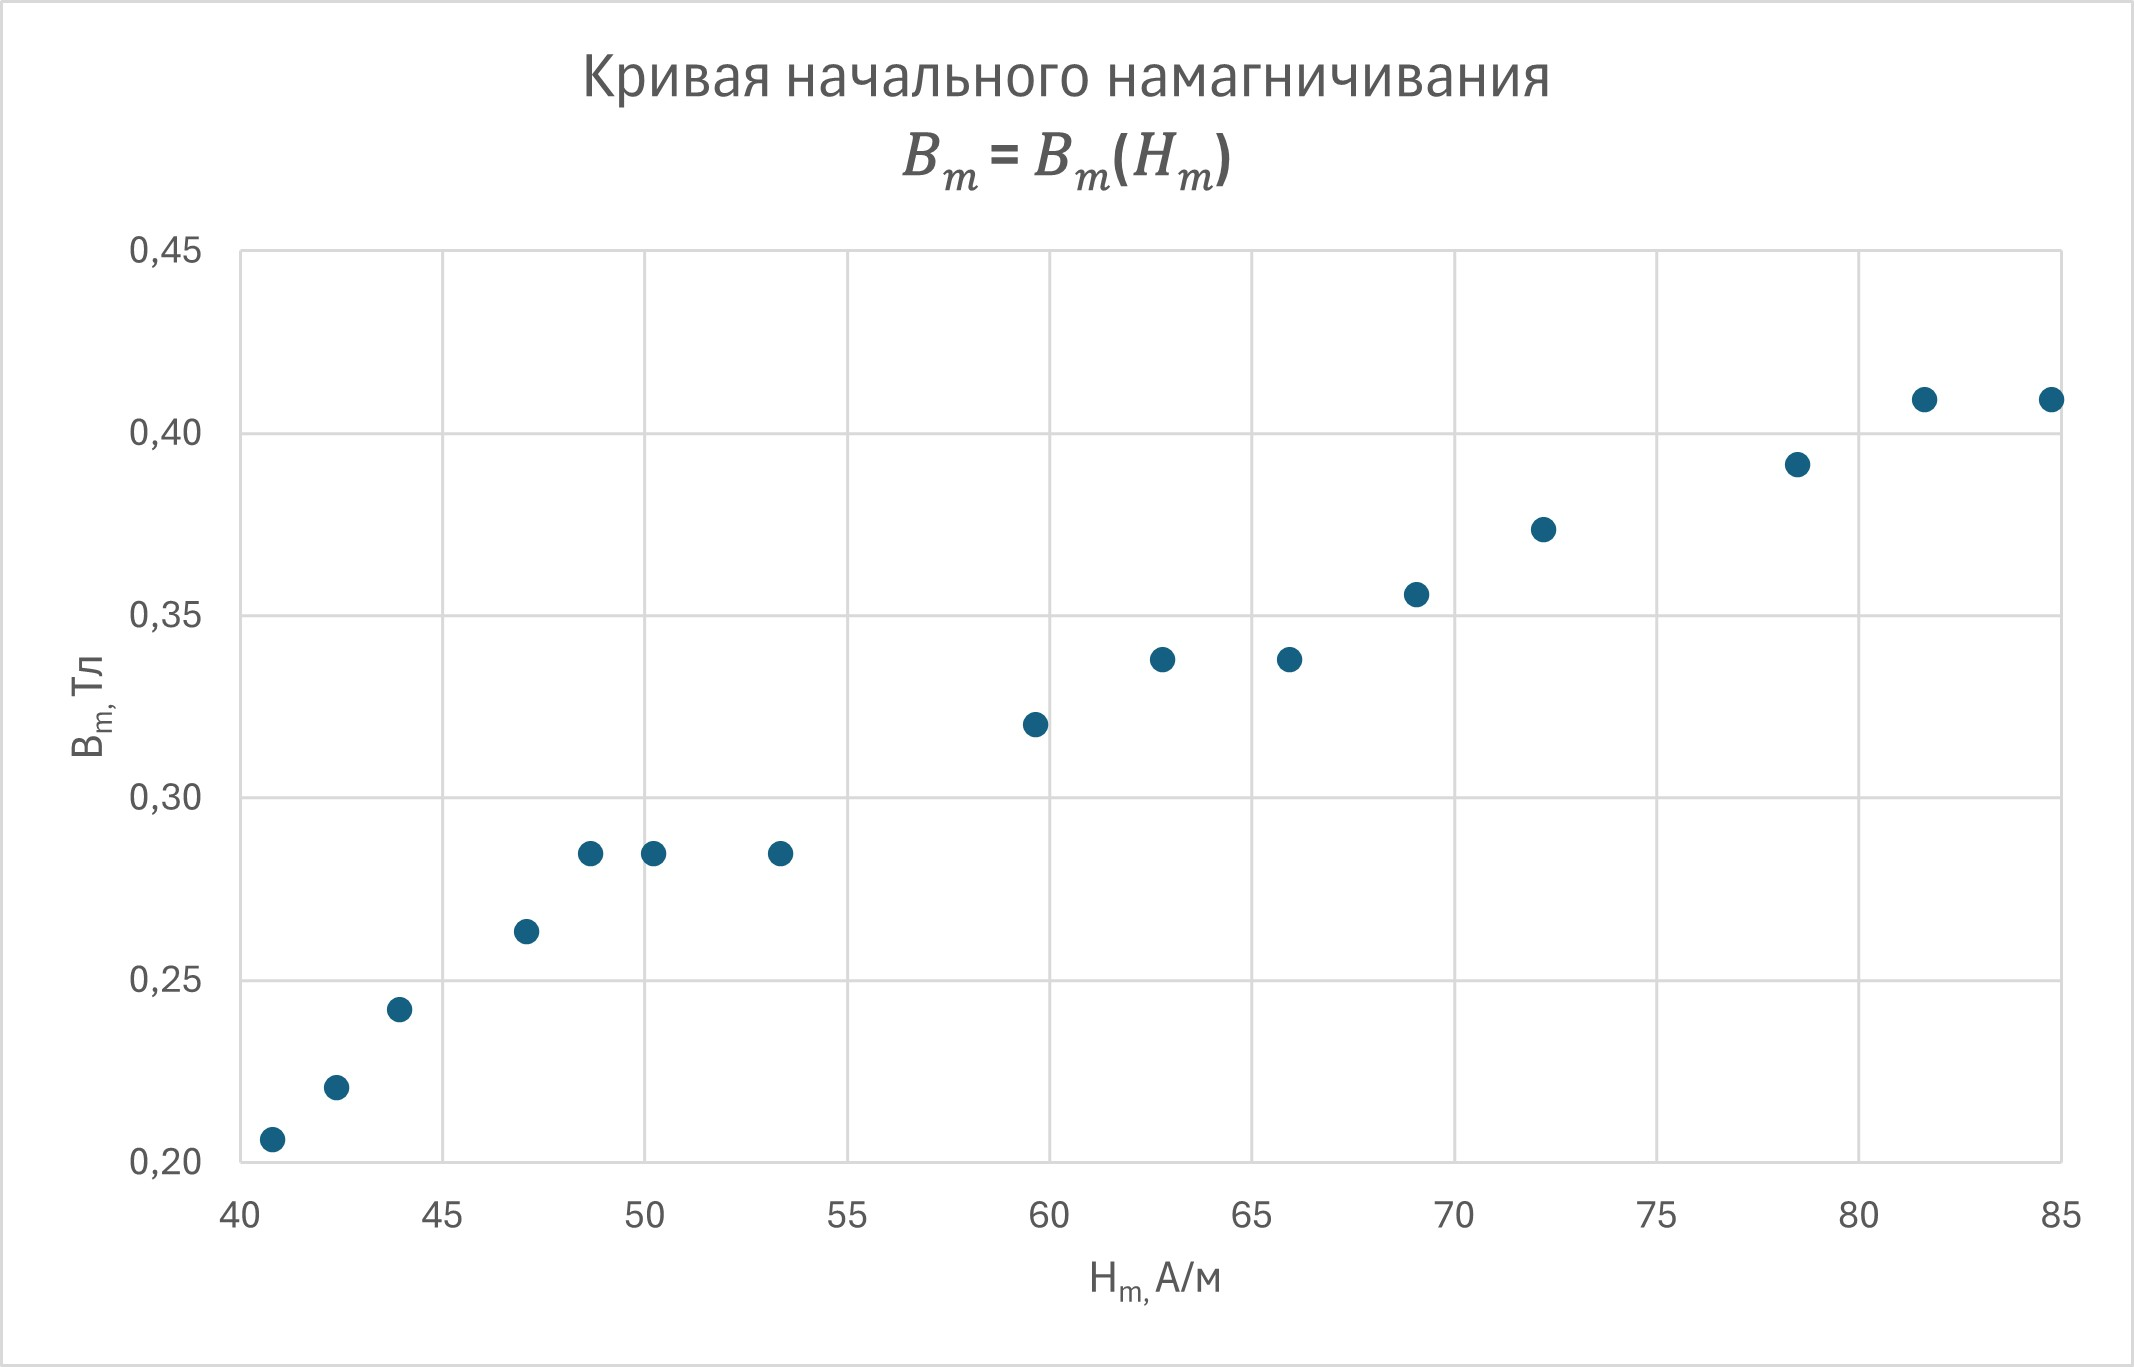
\includegraphics[width=15cm]{images/B_m.jpg}

    \smallvspace

    \textit{График 1.} Кривая начального намагничивания $B_m = B_m(H_m)$
\end{center}

\hypertarget{diagram2}{}

\begin{center}
    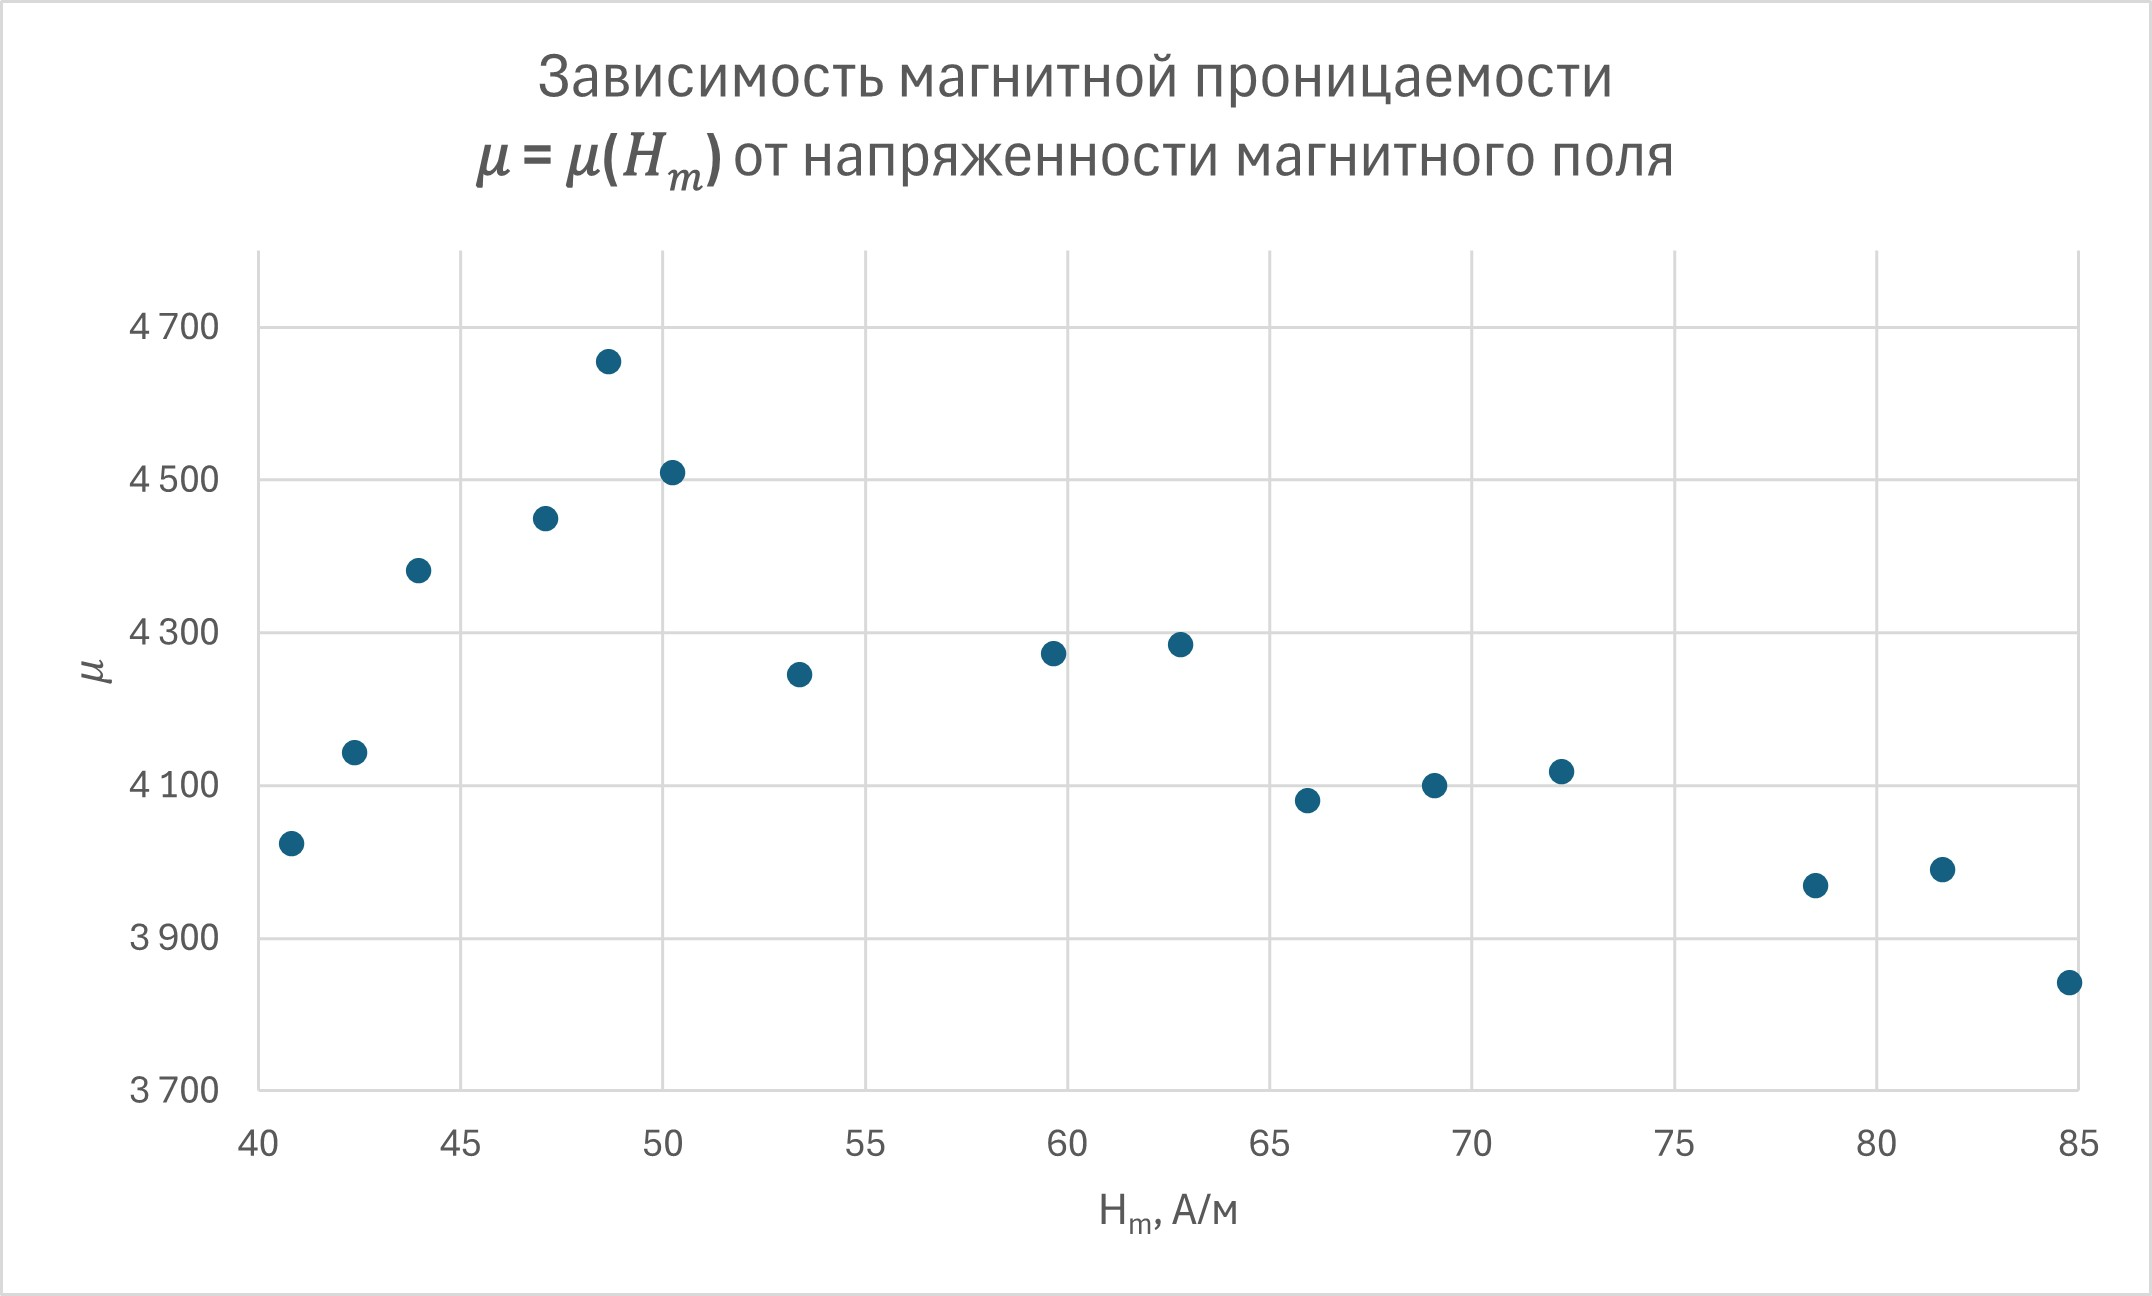
\includegraphics[width=15cm]{images/mu.jpg}

    \smallvspace

    \textit{График 2.} Зависимость магнитной проницаемости $\mu = \mu(H_m)$ от напряженности магнитного поля
\end{center}

\hypertarget{diagram3}{}

\begin{center}
    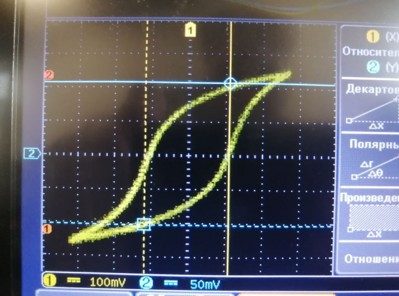
\includegraphics[width=15cm]{images/petlya_1.jpg}

    \smallvspace

    \textit{График 3.} Петля гистерезиса ферромагнетика
\end{center}

\hypertarget{diagram4}{}

\begin{center}
    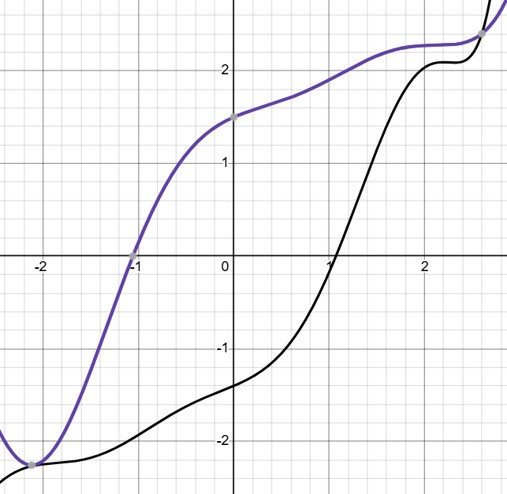
\includegraphics[width=12cm]{images/petlya_2.jpg}

    \smallvspace

    \textit{График 4.} Интерполяция петли гистерезиса ферромагнетика
\end{center}


\end{document}